\documentclass[12pt,a4paper]{article}
\usepackage[utf8]{inputenc}
\usepackage{amsmath}
\usepackage{amsfonts}
\usepackage{amssymb}
\usepackage{float}
\usepackage{csvsimple}
\usepackage{enumerate}
\usepackage{hyperref}
\usepackage{graphicx}
\usepackage{gensymb}
\usepackage{txfonts}
\usepackage{listings}
\usepackage{cleveref}
\usepackage{xcolor}
\parindent 0px
\usepackage[none]{hyphenat}
\usepackage{listings} %Package for the enviroment in which we write code 
\usepackage[left=1cm,right=1cm,top=2cm]{geometry}
\pagenumbering{arabic}
%Some custom colours
\definecolor{codegreen}{rgb}{0,0.6,0}
\definecolor{codegray}{rgb}{0.5,0.5,0.5}
\definecolor{codepurple}{rgb}{0.58,0,0.82}
\definecolor{backgroundcolour}{rgb}{0.95,0.95,0.92}

%Shortcut for strings "Code" and "List of Code"
\renewcommand{\lstlistingname}{Code}
\renewcommand{\lstlistlistingname}{List of Code}

%This is the template for code styling, named as "mystyle"
\lstdefinestyle{mystyle}{
	backgroundcolor=\color{backgroundcolour},
	basicstyle=\ttfamily\small,
	commentstyle=\color{green!60!black},
	keywordstyle=\color{magenta},
	stringstyle=\color{blue!50!red},
	showstringspaces=false, 
	captionpos=b, %Position of caption top/bottom
	%numbers=left,	%This command adds line numbers to the code
	%numberstyle=\footnotesize\color{gray}, %This command sets the colour of the line numbers
	%numbersep=10pt, %This command determines the separation of the line numbers from the main margin
	%stepnumber=2,
	tabsize=2,
	frame=single, %setting to select the frame for code ... options available {L,single,shadowbox}
	%framerule=1pt, %selecting the width of the frame
	%rulecolor=\color{red}, %selecting the colour of the frame
	breaklines=true,
	inputpath=code
}

%%%%%%%%%%%%%%%%%%%%%%%%%%%%%%%%%%%%%%%%%%%%%%%%%%%%%%%%%%%%%%%%%%%%%%%%%%%%%%%%%%%%%%%%%%%%%%%%%%%%%%%%%%%%%%%%%%%%%%%%%%%%%%%%%%%%%%%%%%%%%%%%%%%%%%%%%%%%%%%%%%%%%%%%%%%%%%%%%%%%%%%%%%%%%%%%%%%%%%%%%%%%%%%%%%%%%%%%%%%%%%
\title{OPERATING SYSTEMS \\ SEMAPHORES SYNCHRONISATION}
\author{ANUDEEP RAO PERALA}
\date{}

\begin{document}
	\maketitle
	
	\tableofcontents
	\newpage
	
	\section{Goal :}
	\begin{itemize}
		\item Using semaphores to synchronize the $P$ passenger processes and the $C$ car processes and analyzing average time of riding for each person based on changing values of $P$, $C$.
	\end{itemize}
	\section{Input :}
	\begin{itemize}
		\item Input is the set of numbers:
		\begin{enumerate}
			\item Number of Passenger threads ($P$)
			\item Number of Cars $(C)$
			\item Mean value of exponential wait time between 2 successive ride requests made by the passenger $(\lambda _P)$
\item Mean value of exponential wait time between 2 successive ride request accepted by a car $(\lambda _C)$
		\end{enumerate}
		
	\end{itemize}
	\section{Output :}
	\begin{itemize}
		\item The output data is written to output file $output.txt$ which contains all log for all the rides.
	\end{itemize}
	
	\section{Procedure :}
	\begin{itemize}
	\item Input is read from the file \textbf{input.txt} and stored in variables:
	\begin{enumerate}
		\item $P$ - stores Passengers value
		\item $C$ - stores Consumers value
		\item $lamb_1$ - stores value of $\lambda_1$
		\item $lamb_2$ - stores value of $\lambda_2$
		\item $K$ - stores value of number of ride requests by each passenger
	\end{enumerate}
	\begin{lstlisting}[language=C++, style = mystyle]
	int P = 0; 
	int C = 0; 
	int lamb1 = 0;
	int lamb2 = 0;
	int K = 0;
\end{lstlisting}
	\item The mutex variables: 
\begin{enumerate}
	\item \textbf{ret} - This vector array stores all the strings outputted from the program which are needed to be written to the \textbf{output.txt} file.
	\item \textbf{cars\_availability} - The array which keeps track of which car is free, and which car is already in ride. 
	\item \textbf{mtx\_writing} - is used for locking when there is a new string addition to the vector array \textbf{ret} is done.
	\item \textbf{sem\_array} - This is a counting semaphore, which works based on the number of cars free for ride.
	\item \textbf{total\_time\_passengers} - This adds up the total time for the whole process execution for each passenger, then we use it for calculating the average time for each set of $(P,C,\lambda_1,\lambda_2,K)$
	\item \textbf{total\_time\_cars} - This adds up the total time for the whole process execution for each car, then we use it for calculating the average time for each set of $(P,C,\lambda_1,\lambda_2,K)$

\end{enumerate}
	\begin{lstlisting}[language=C++, style = mystyle,label={lst:2}]
	vector<string> ret;
	int *cars_availability;
	pthread_mutex_t mtx_writing;      
	sem_t *sem_array;                 
	double total_time_passengers = 0;  
	double total_time_cars = 0;  
	\end{lstlisting}

	\item This structure is used to send arugument to the $passenger()$ whose parameters are :
\begin{enumerate}
	\item \textbf{passenger\_number} - This varable stores the serial number of passenger 
	\item  \textbf{cars} - This is the array which has the thread ID's of the cars threads.
	\item \textbf{attr} - The default paramter for thread creation
\end{enumerate}
	\begin{lstlisting}[language=C++, style = mystyle]
	struct data_to_passenger_func
	{
		int passenger_number; 
		pthread_t *cars;   
		pthread_attr_t attr;
	};
	typedef struct data_to_passenger_func parampass;
\end{lstlisting}
	\item This structure is used to send arugument to the $cars()$ whose parameters are :
\begin{enumerate}
	\item \textbf{car\_number} - This varable stores the serial number of car in use by the current passenger.
	\item  \textbf{passenger\_number} - This varable stores the serial number of passenger 
	\item \textbf{time\_sleep} - This is the time for which the car thread sleeps so that the given constraint of not accepting new request is satisfied
\end{enumerate}
	\begin{lstlisting}[language=C++, style = mystyle]
	struct data_to_car_func
	{
		int car_number;      
		int passenger_number; 
		double time_sleep;   
	};
	typedef struct data_to_car_func paramcar;
\end{lstlisting}

	\item The following code block corresponds to all the intialization of mutex, semaphore variable and the availability array for the cars.
	\begin{lstlisting}[language=C++, style = mystyle]
// intializing the mutex variable
	pthread_mutex_init(&mtx_writing, nullptr);

// initializing semaphore variable to cars count
	sem_array = sem_open("/arraysem", O_CREAT | O_EXCL, 0644, C);

// initializing the cars availability array
	cars_availability = (int *)calloc(C, sizeof(int));
	for (int i = 0; i < C; i++)
		cars_availability[i] = 1;
\end{lstlisting}

	\item Creating passenger threads, with the pointer variable of \textbf{parampass struct} being passed as argument with suitable values loaded in.
\item Control of program is now shifted from $main()$ to $passengers()$.
	\begin{lstlisting}[language=C++, style = mystyle]
	pthread_t passengers[P]; // This is the thread pool of passengers
	pthread_t cars[C];       // This is the thread pool of cars
	pthread_attr_t attr;
	pthread_attr_init(&attr);

	for (int i = 0; i < P; i++)
 		{
	   		auto *dat = (parampass *)calloc(1, sizeof(parampass));
	   		dat->passenger_number = i + 1;
	   		dat->cars = cars;
	   		dat->attr = attr;
	   		pthread_create(&passengers[i], &attr, passenger, dat);
    	}
\end{lstlisting}

	\item The following code block is used for generation of the random times used in the program in the critical section of $passenger()$ and $cars()$ threads.
	\begin{lstlisting}[language=C++, style = mystyle]
	int seed = chrono::system_clock::now().time_since_epoch().count();
    default_random_engine generator(seed);
    exponential_distribution<double> t_1(1.0 / lamb1);
    exponential_distribution<double> t_2(1.0 / lamb2);

    double t1 = t_1(generator);
    double t2 = t_2(generator);
\end{lstlisting}

	\item We use the mutex lock \textbf{mtx\_writing}, whenever we want to add a string value to the vector array \textbf{ret}.
		\begin{lstlisting}[language=C++, style = mystyle]
	pthread_mutex_lock(&mtx_writing);
		/*
			Adding a new string to ret vector array
		*/
	pthread_mutex_unlock(&mtx_writing);
	\end{lstlisting}
	
	\item Whenever we want to find the local time the above code block is used. From the variable \textbf{timeinfo} we can get the required info about local time by accessing the struct data. 
		\begin{lstlisting}[language=C++, style = mystyle]
	time_t raw_time;
	struct tm *timeinfo;
  	time(&raw_time);
	timeinfo = localtime(&raw_time);
\end{lstlisting}

	\item The following code block is the entry section for the passenger thread.
\item The semaphore variable \textbf{sem\_array} ensures that a passenger thread can only access the \textbf{car\_availability} array when  there is a car available for riding i.e.,  \textbf{sem\_array}$>0$.
\item After crossing the $sem\_wait()$ function search for a free car is done, after finding it the index of car it is stored in variable \textbf{index\_car} variable which is then passed on to thread function $cars()$.
\item After loading required values to argument for passing we create a car thread with the \textbf{pthread\_t} variable \textbf{dat$->$cars[index\_car]}.
		\begin{lstlisting}[language=C++, style = mystyle]
// Entry section of the passenger thread
	for (int j = 0; j < K; j++)
	{
		int index_car = 0;
// Blocked this section inorder to remove race conditions
// for array value choosing
		sem_wait(sem_array); 
		for (int i = 0; i < C; i++)
		{
			if (cars_availability[i] == 1)
			{
				index_car = i;
				cars_availability[i] = 0;
				break;
			}
		}
	
	paramcar *a = (paramcar *)calloc(1, sizeof(paramcar));
	a->passenger_number = dat->passenger_number;
	a->car_number = index_car + 1;
	a->time_sleep = t2;
	pthread_create(&dat->cars[index_car], &dat->attr, cars, a);
	pthread_join(dat->cars[index_car], nullptr]);
	cars_availability[index_car] = 1;
	sem_post(sem_array); // Incrementing the sem_array value
\end{lstlisting}


	\item Now here the program control shifts from $passengers()$ to $cars()$.
	
	\item The following code block is the Entry Section and CS of the car thread.
	\item The sleep time is in $\mu$ sec.
			\begin{lstlisting}[language=C++, style = mystyle]
// Entry section for car thread
	pthread_mutex_unlock(&mtx_writing);

// CS for car thread
	usleep(d->time_sleep*1000);
		\end{lstlisting}
		
	\item We use the following code block to calculate time of execution of an action.
	\item The output time is in $\mu$ seconds.
			\begin{lstlisting}[language=C++, style = mystyle]
	auto start = high_resolution_clock::now(); 
/*
	The required action is performed 
*/
    auto stop = high_resolution_clock::now(); 
	auto timees = duration_cast<microseconds>(stop - start); 
	cout << (double)timees.count() ; 
\end{lstlisting}
	\item After execution of Remainder Section control of the program shifts from $cars()$ to $passengers()$.
\item The function $pthread\_join()$ ensures that the $car$ thread is executed fully.
\item Then the \textbf{cars\_availibity} arrays value is resette to $1$. Then semaphore value is incremented using $sem\_post()$.
			\begin{lstlisting}[language=C++, style = mystyle]
	pthread_join(dat->cars[index_car], nullptr);
    cars_availability[index_car] = 1;
    sem_post(sem_array); 
\end{lstlisting}
\item The  critical section of passenger depends on $t_1,\, t_2$ if $t_1>t_2$ then we need to still wait for a time of $t_1-t_2$, for the passenger to pass new request to a car. But when $t_1<t_2$, in this case as already the passenger has passed the time $t_1$ passenger can putforth a new request as soon as the passeger exits the car.
			\begin{lstlisting}[language=C++, style = mystyle]
// CS of passenger thread
	if (t1 > t2)
	usleep((int)(t1-t2)*1000);
\end{lstlisting}

\item The average Time of execution of Passengers and Cars is calculated like as shown below.
				\begin{lstlisting}[language=C++, style = mystyle]
cout << "Total avg time of execution of passengers is in secs : " <<
 								total_time_passengers / P << endl;
cout << "Total avg time of execution of cars is in secs : " <<
								 total_time_cars / C << endl;
\end{lstlisting}

\item File writing is done with the global vector array \textbf{ret}.
\item The output to file is not in the order that was mentioned in the problem statement, this was done in purpose inorder to prove the concurrency of the program.
\item In the output file the system time of the output can be seen it will not change this is because as we considered the sleep times in milli seconds.
 				\begin{lstlisting}[language=C++, style = mystyle]
	ofstream op;
	op.open("output.txt", ios_base::out);
   for (const auto & i : ret)
	{	
		op << i;
	}
	\end{lstlisting}
\end{itemize}

	\section{ Analyzing Program Output :} 
	
	\begin{itemize}
		\item We analyze the program in two modes:
		\begin{enumerate}
			\item $T_{avg}$ for passengers to complete their tour with Total number of Cars as constant ($C$ is constant).
			\item $T_{avg}$ for Cars to complete their tour with Total number of Passengers as constant ($P$ is constant).
		\end{enumerate}
	\end{itemize}
	
	\subsection{$C$ is constant :}
	\begin{itemize}
		\item The value of $C$ used by the program is fixed and is equal to $25$.
		\item The value of $K$ used by the program is equal to $5$
		\item $\lambda _1$ is equal to $10$
		\item $\lambda _2$ is equal to $10$
	\end{itemize}
	
	\subsubsection{Graph :}
	\begin{figure}[H]
		\centering
		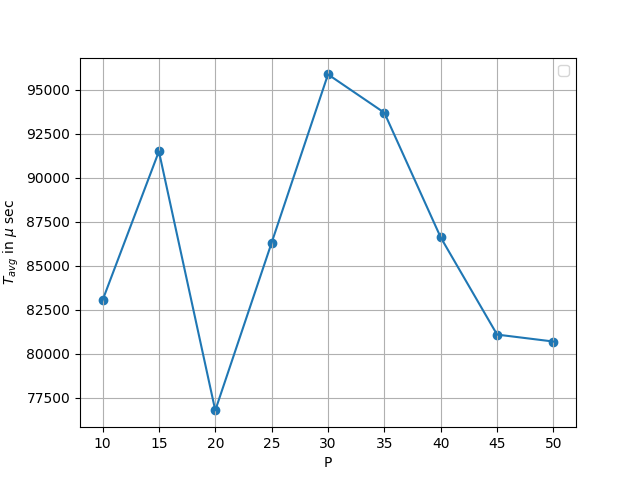
\includegraphics[width=0.9\textwidth]{C_const}
		\caption{$T_{avg}$ vs $P$ ($C$ is constant)}
	\end{figure}

	\subsubsection{Observations :}
	\begin{itemize}
		\item \underline{\textbf{Expected}} : 
		\begin{itemize}
			\item As the value of $P$ increases $T_{avg}$ should increase as $C$ is constant waiting time of each passenger increases.
		\end{itemize}
		\item \underline{\textbf{Observed}} : 
		\begin{itemize}
			\item We observe some unusual trend in the $T_{avg}$ of this case.
			\item We see that there isn't much difference between the average times between the values of $P=10$ to $P=25$ which is because of the fact that the value of $C=25$ we have more cars than passengers, because of this the time differences are not much high in this range of $P$, i.e., the waiting time isn't that high.
			\item The value of $T_{avg}$ increases as expected in $P=20$ to $P=30$.
			\item Except for the values at $P=20$ and $P=30$ all other $T_{avg}$ are nearly at the same times, as we are measuring the time in $\mu$ seconds.
			\item This irregular time variations can be attributed to hardware implementation of the PC.
		\end{itemize}
	\end{itemize}
	
	\subsection{$P$ is constant :}
	\begin{itemize}
	\item The value of $P$ used by the program is fixed and is equal to $50$.
	\item The value of $K$ used by the program is equal to $3$
	\item $\lambda _1$ is equal to $10$
	\item $\lambda _2$ is equal to $10$
\end{itemize}

	\subsubsection{Graph :}
	    \begin{figure}[H]
		\centering
		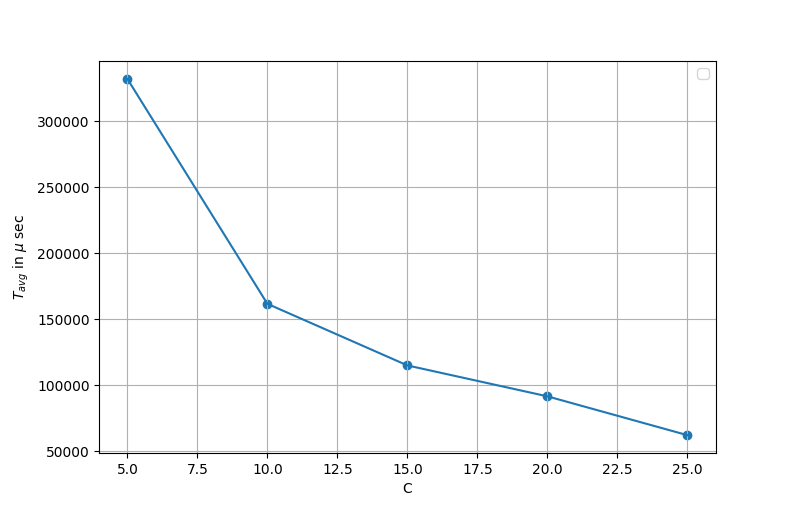
\includegraphics[width=1\textwidth]{P_const}
		\caption{$T_{avg}$ vs $C$ ($P$ is constant)}
	    \end{figure}

	\subsubsection{Observations :} 
	\begin{itemize}
		\item \underline{\textbf{Expected}} : 
		\begin{itemize}
			\item As the value of $C$ increases the average working time decreases.
		\end{itemize}
		\item \underline{\textbf{Observed}} : 
		\begin{itemize}
			\item As the value of $C$ increases $T_{avg}$ decreases, which follows the expected pattern.
			\item This is because as the number of cars increases work load on each car decreases which inturn decreases the time of ride for each car which results in decrease of $T_{avg}$. 
		\end{itemize}
	\end{itemize}  		
	
\end{document}



